\global\addtocounter{part}{-1}%
\part[author={\protect\insertauthor},label={chap:moduleoverview}]{Overview of the module DA53}

\begin{graphicspathcontext}{{./chapters/chapter0/imgs/raw/},{./chapters/chapter0/imgs/auto/}{./chapters/appendix/imgs/raw/}}
		
\begin{frame}{Prof\string.dr\string. St\'ephane GALLAND}
	\begin{minipage}[t]{.75\linewidth}
		\begin{raggedright}
			\textit{Full Professor} \\[.5cm]
			{\scriptsize
				Universit\'e de Technologie de Belfort-Montb\'eliard, France \\
				Director of the CIAD Laboratory} \\[.25cm]
			\textbf{Topics: Multiagent systems, Agent-based simulation, Agent-oriented software engineering, Mobility and traffic modeling} \\[.5cm]
		\end{raggedright}
	\end{minipage}%
	\hfill%
	\raisebox{-\height}{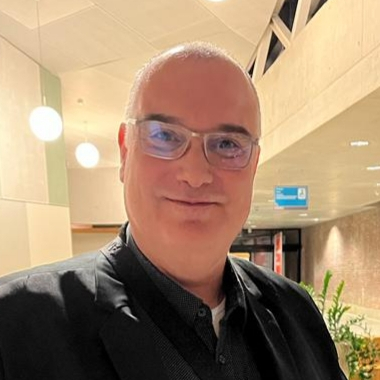
\includegraphics[width=2cm]{sgalland}} \\[.5cm]%
	\begin{raggedright}
		\scriptsize \begin{tabularx}{\linewidth}{@{}lX@{}}
			Web page: & \url{http://www.ciad-lab.fr/stephane_galland/} \\
			Email: & \href{mailto:stephane.galland@utbm.fr}{stephane.galland@utbm.fr} \\
		\end{tabularx} \\[.5cm]
		\scriptsize Open-source contributions:\begin{itemize}\tiny
			\item \url{http://www.sarl.io}
			\item \url{http://www.janusproject.io}
			\item \url{http://www.aspecs.org}
			\item \url{http://www.arakhne.org}
			\item \url{https://github.com/gallandarakhneorg/}
		\end{itemize}
	\end{raggedright}
\end{frame}

\begin{frame}{Goals of this module}
	\begin{leftanchorblock}{}{1}
		Study models, techniques and algorithms that permit to analyze a text-based language
	\end{leftanchorblock}
	\vspace{0.5cm}
	\begin{rightanchorblock}{}{2}
		Study models, techniques and algorithms that permit to generate and execute code
	\end{rightanchorblock}
	\begin{leftanchorblock}{}{3}
		Study the techniques for the optimization of executable codes \alert{(available soon)}
	\end{leftanchorblock}
\end{frame}

\tableofcontentslide[onlyparts]

\section{Recommendations}

\begin{frame}{Recommended Knowledge}
	\fancybox{Object Oriented Programming}{Java, C\#, C++, Python}{oop}{1}
	\hfill
	\fancybox{CLI Compilation}{Java, g++, Maven, Make}{cli}{2}
	\hfill
	\fancybox{Algorithms}{Statements, Data structures}{algorithm}{3}
\end{frame}

\begin{frame}{{Best Way} to Follow the Lectures}
	\begin{columns}
		\begin{column}{.5\linewidth}
			\begin{rightanchorblock}{}{1}
				Download the PDF files of the slides before the lecture
			\end{rightanchorblock}
			\begin{rightanchorblock}{}{2}
				Do not read \emph{each word} of the slides during the lectures
			\end{rightanchorblock}
			\begin{rightanchorblock}{}{3}
				Listen carefully the teachers and takes notes on the side of the slides
			\end{rightanchorblock}
		\end{column}
		\begin{column}{.5\linewidth}
			\begin{leftanchorblock}{}{4}
				Ask questions \dots Ask questions \dots Ask questions
			\end{leftanchorblock}
			\vspace{.5cm}
			\begin{leftanchorblock}{}{5}
				You must read the slides at home as soon as possible, not few hours before the exams
			\end{leftanchorblock}
		\end{column}
	\end{columns}
\end{frame}

\section{Module organization}

\begin{leftlawnframe}{{Another Yet} English Module}{lawnenglishcourse}
	Lectures \pgfuseimage{small-english-flag} \\[.5cm]
	Supervised tutorials \pgfuseimage{small-english-flag} [\pgfuseimage{small-french-flag}] \\[.5cm]
	Laboratory works \pgfuseimage{small-english-flag} [\pgfuseimage{small-french-flag}] \\[.5cm]
	Exams \pgfuseimage{small-english-flag}
\end{leftlawnframe}

\begin{gridframe}{Evaluation of the Students}
	\cell2{final-exam}{\large Mid-Term Exam $30\%$}
	\cell4{final-exam}{\large Final Exam $30\%$}
	\cell8{laboratory-works}{\large Laboratory works $40\%$}
	\cell{10}{project-eval}{\large Project --- see DA50}
\end{gridframe}

\begin{frame}[background=6]{Tools}
	\begin{block}{Languages}
		\begin{itemize}
			\item Java --- tutorials and projects
			\item C/C++/C\# --- projects
		\end{itemize}
	\end{block}
	\begin{block}{Integrated Development Environment}
		\begin{itemize}
			\item Eclipse --- tutorials and projects
			\item NetBean, IntelliJ, Visual Studio --- projects
		\end{itemize}
	\end{block}
	\begin{block}{Compilation Tools}
		\begin{itemize}
			\item javacc --- tutorials, projects
			\item Xtext --- projects
			\item jlex, lex, flex, yacc, bison --- projects
		\end{itemize}
	\end{block}
\end{frame}

\section{Books}

\libraryslide[frametitle={Recommended Book},subtitle={2nd edition}]{book1}{Compilers --- Principles, Techniques and Tools
Second Edition}{Alfred V. AHO, Monica S. LAM, Ravi SETHI and Jeffrey D. ULLMAN}{Pearson \& Addison Wesley, 2007}{0-321-48681-1}

\libraryslide[frametitle={Recommended Book}]{book2}{Parsing Techniques --- A Practical Guide}{Dick Grune and Ceriel J.H. Jacobs}{Springer Verlag New York, 2007}{0-387-20248-X}

\libraryslide[frametitle={Recommended Book}]{book3}{Calculabilité, Complexité et Approximation}{Jean-François REY}{Vuibert, France, 2004}{2-7117-4808-1}

\end{graphicspathcontext}
